\documentclass[a4paper, 11pt]{article}
    \usepackage{comment} % enables the use of multi-line comments (\ifx \fi) 
    \usepackage{lipsum} %This package just generates Lorem Ipsum filler text. 
    \usepackage{fullpage} % changes the margin
    \usepackage{CJKutf8}
    \usepackage{enumitem}
    \usepackage{titlesec}
    \usepackage{graphicx}     % for figure
    \usepackage{subcaption}   % for figure
    \usepackage[export]{adjustbox}
    \usepackage[most]{tcolorbox}
    \usepackage{xcolor}
    \usepackage{multicol}
    \usepackage{array}
    \usepackage{wrapfig}
    \usepackage{multirow}
    \usepackage{tabu}
    \usepackage{hyperref}
    % For tree
    \usepackage{tikz}
% \renewcommand{\theenumi}{(\alph*)}
  \usepackage{mathtools}

\DeclarePairedDelimiter\ceil{\lceil}{\rceil}
\DeclarePairedDelimiter\floor{\lfloor}{\rfloor}

\titlespacing*{\section}
  {0pt}{0.5\baselineskip}{1\baselineskip}

\titlespacing*{\subsection}
  {0pt}{0.1\baselineskip}{0.1\baselineskip}

\begin{document}
%Header-Make sure you update this information!!!!
\noindent
\begin{center}
  \large\textbf{2018 Fall Data Compression Homework \#1} \\
\end{center}
\begin{CJK}{UTF8}{bsmi}
\normalsize EE 248583 \hfill \textbf{106368002 張昌祺 Justin, Chang-Qi Zhang} \\
Advisor: 電子所 高立人 副教授 \hfill justin840727@gmail.com \\
\null\hfill Due Date: November 12 2018 \\
\end{CJK}

\section*{Problem 1 Entropy}
Let X be a random variable with an alphabet $H=\{1, 2, 3, 4, 5\}$. Please determine 
$H(X)$ for the following three cases of probability mass function $p(i)=prob[X=i]$.~(15\%)
\begin{enumerate}[label=(\alph*)]
  \item $P(1)=P(2)=1/2$:
    \subsection*{Ans}
    \begin{align*}
      H(X)&=-(P(1)\log_{2}P(1)+P(2)\log_{2}P(2)) \\
          &=-(0.5\log_{2}(0.5)+0.5\log_{2}(0.5)) \\
          &=-(-0.5-0.5)  \\
          &=1 ~bits/symbol
    \end{align*}
    \label{p:1-a}
  \item $P(i)=1/4, for~i = 1, 2, 3,and~p(4) = p(5) = 1/8$:
    \subsection*{Ans}
    \begin{align*}
      H(X)&=-(3\times P(1)\log_{2}P(1)+P(4)\log_{2}P(4)+P(5)\log_{2}P(5)) \\
          &=-(3\times 0.25\log_{2}(0.25)+2\times 0.125\log_{2}(0.125)) \\
          &=-(-1.5-0.75)  \\
          &=2.25 ~bits/symbol
    \end{align*}
    \label{p:1-b}
  \item $P(i)=2^{-i}, for~i = 1, 2, 3, 4,and~p(5) =  1/16$:
    \subsection*{Ans}
    \begin{align*}
      H(X)&=-(\sum_{i=1}^{4} 2^{-i}\log_{2}2^{-i}+\frac{1}{16}\log_{2}\frac{1}{16}) \\
          &=-(0.5\times(-1)+0.25\times(-2)+0.125\times(-3)+0.0625\times(-4)
            +0.0625\times(-4)) \\
          &=1.875 ~bits/symbol
    \end{align*}
    \label{p:1-c}
\end{enumerate}
\newpage
\section*{Problem 2 Huffman Code}
Design a Huffman code C for the source in Problem 1. (15\%)
\begin{enumerate}[label=(\alph*)]
  \item Specify your codewords for individual pmf model in Problem 1.
  \subsection*{Ans}
  \textbf{1.\ref{p:1-a}}
  \begin{multicols}{2}
    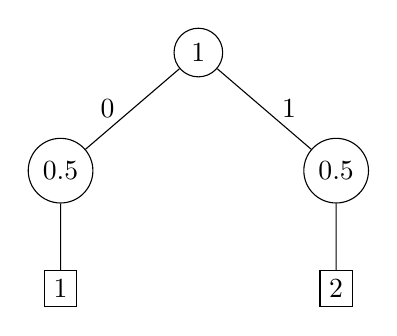
\begin{tikzpicture}[level distance=1.5cm,
      level 1/.style={sibling distance=3.5cm},
      level 2/.style={sibling distance=1cm}]
      \tikzstyle{every node}=[circle,draw]
      \node (Root) {1}
      child {
          node  {$0.5$} 
          child { node[rectangle] {1}}
          edge from parent node[left,draw=none] {0}
      }
      child {
          node {$0.5$}
          child { node[rectangle] {2} }
          edge from parent node[right,draw=none] {1}
      };
      % \noindent
      \end{tikzpicture} 
      \columnbreak

      \null \vfill
      \begin{tabular}{ |c|c|c| } 
        \hline
        Alphabet & P  & Codeword \\
        \hline
        1 & 0.5 & 0 \\ 
        2 & 0.5 & 1 \\  
        \hline
        \end{tabular}

        \null \vfill
  \end{multicols}
  \vspace{5em}
  \textbf{1.\ref{p:1-b}}
  \begin{multicols}{2}
    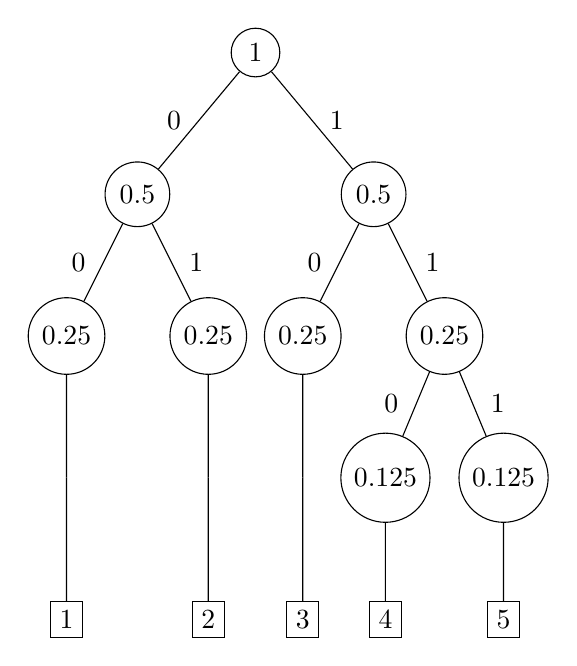
\begin{tikzpicture}[level distance=1.8cm,
      level 1/.style={sibling distance=3.0cm},
      level 2/.style={sibling distance=1.8cm},
      level 3/.style={sibling distance=1.5cm}]
      \tikzstyle{every node}=[circle,draw]
      \node (Root) {1}
      child {
        node {$0.5$} 
        child { node {$0.25$
        } 
        child{child{node[rectangle] {1}}}
        edge from parent node[left,draw=none] {0}
        }
        child { node {$0.25$} 
        child{child{node[rectangle] {2}}}
        edge from parent node[right,draw=none] {1}
        }
        edge from parent node[left,draw=none] {0}
      }
      child {
        node {$0.5$}
        child { node {$0.25$} 
          child{child{node[rectangle] {3}}}
          edge from parent node[left,draw=none] {0}
        }
        child { node {$0.25$}
          child { node {$0.125$} 
            child{node[rectangle] {4}}
            edge from parent node[left,draw=none] {0}
          }
          child { node {$0.125$} 
            child{node[rectangle] {5}}
            edge from parent node[right,draw=none] {1}
          } 
            edge from parent node[right,draw=none] {1}
        }
        edge from parent node[right,draw=none] {1}
      };
      % \noindent
      \end{tikzpicture} 
      \columnbreak
        
      \null \vfill
      \begin{tabular}{ |c|c|l| } 
        \hline
        Alphabet & P & Codeword \\
        \hline
        1 & 0.25  & 00  \\ 
        2 & 0.25  & 01  \\
        3 & 0.25  & 10  \\
        4 & 0.125 & 110 \\
        5 & 0.125 & 111 \\
        \hline
        \end{tabular}

        \null \vfill
  \end{multicols}
  \newpage
  \textbf{1.\ref{p:1-c}}
  \begin{multicols}{2}
    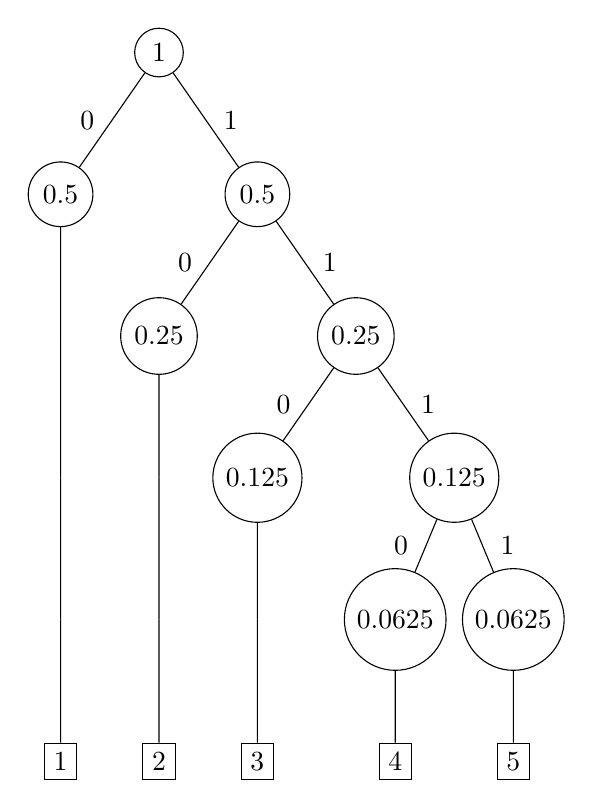
\begin{tikzpicture}[level distance=1.8cm,
      level 1/.style={sibling distance=2.5cm},
      level 2/.style={sibling distance=2.5cm},
      level 3/.style={sibling distance=2.5cm},
      level 4/.style={sibling distance=1.5cm}]
      \tikzstyle{every node}=[circle,draw]
      \node (Root) {1}
      child {
          node {$0.5$} 
          child { 
            child {
              child {
                child {
                  node[rectangle] {1}
                }
              }
            }
          }
          edge from parent node[left,draw=none] {0}
      }
      child {
          node {$0.5$}
          child { node {$0.25$} 
            child { 
              child {
                child {
                  node[rectangle] {2}
                }
              }
            }
            edge from parent node[left,draw=none] {0}
          }
          child { node {$0.25$}
            child { node {$0.125$}
              child { 
                child {
                    node[rectangle] {3}
                }
              }
              edge from parent node[left,draw=none] {0}
            }
            child { node {$0.125$}
              child { node {$0.0625$}
                child {
                  node[rectangle] {4}
                }
                edge from parent node[left,draw=none] {0}
              }
              child { node {$0.0625$}
                child {
                  node[rectangle] {5}
                }
                edge from parent node[right,draw=none] {1}
              }
              edge from parent node[right,draw=none] {1}
            }
            edge from parent node[right,draw=none] {1}
          }
          edge from parent node[right,draw=none] {1}
      };
      % \noindent
      \end{tikzpicture}
      \columnbreak

      \null \vfill
      \begin{tabular}{ |c|c|l| } 
        \hline
        Alphabet & P  & Codeword \\
        \hline
        1 & 0.5     & 0 \\ 
        2 & 0.25    & 10 \\  
        3 & 0.125   & 110 \\  
        4 & 0.0625  & 1110 \\  
        5 & 0.0625  & 1111 \\  
        \hline
        \end{tabular}

        \null \vfill
  \end{multicols}
  \vspace{2em}
  \item Compute the expected codeword length and compare with the entropy for your codes in (a).
  \subsection*{Ans}
  \textbf{1.\ref{p:1-b}}
  \begin{align*}
    Expected~codeword~length&=0.5 \times 1 + 0.5 \times 1 \\
                            &=1 ~bits/symbol~\textbf{(Equal Entropy)}
  \end{align*}
  \textbf{1.\ref{p:1-b}}
  \begin{align*}
    Expected~codeword~length&=0.25 \times 2 + 0.25 \times 2 + 0.25 \times 2 + 
                              0.125 \times 3 + 0.125 \times 3 \\
                            &=2.25 ~bits/symbol~\textbf{(Equal Entropy)}
  \end{align*}
  \textbf{1.\ref{p:1-c}}
  \begin{align*}
    Expected~codeword~length&=0.5 \times 1 + 0.25 \times 2 + 0.125 \times 3 + 
                              0.0626 \times 4 + 0.0625 \times 4 \\
                            &=4.125 ~bits/symbol~\textbf{(NOT Equal Entropy)}
  \end{align*}
  \newpage
  \item Design a code with minimum codeword length variance for the pmf model in Problem 1.(b)
  \subsection*{Ans}
  \begin{multicols}{2}
    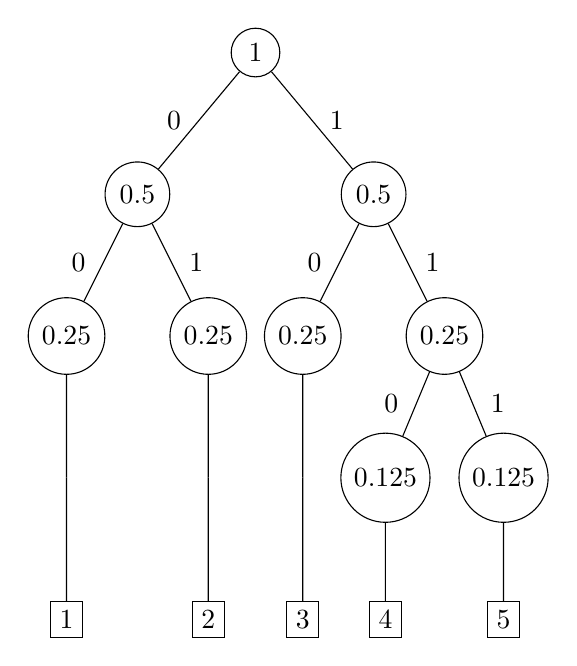
\begin{tikzpicture}[level distance=1.8cm,
      level 1/.style={sibling distance=3.0cm},
      level 2/.style={sibling distance=1.8cm},
      level 3/.style={sibling distance=1.5cm}]
      \tikzstyle{every node}=[circle,draw]
      \node (Root) {1}
      child {
        node {$0.5$} 
        child { node {$0.25$
        } 
        child{child{node[rectangle] {1}}}
        edge from parent node[left,draw=none] {0}
        }
        child { node {$0.25$} 
        child{child{node[rectangle] {2}}}
        edge from parent node[right,draw=none] {1}
        }
        edge from parent node[left,draw=none] {0}
      }
      child {
        node {$0.5$}
        child { node {$0.25$} 
          child{child{node[rectangle] {3}}}
          edge from parent node[left,draw=none] {0}
        }
        child { node {$0.25$}
          child { node {$0.125$} 
            child{node[rectangle] {4}}
            edge from parent node[left,draw=none] {0}
          }
          child { node {$0.125$} 
            child{node[rectangle] {5}}
            edge from parent node[right,draw=none] {1}
          } 
            edge from parent node[right,draw=none] {1}
        }
        edge from parent node[right,draw=none] {1}
      };
      % \noindent
      \end{tikzpicture} 
      \columnbreak
        
      \null \vfill
      \begin{tabular}{ |c|c|l| } 
        \hline
        Alphabet & P & Codeword \\
        \hline
        1 & 0.25  & 00  \\ 
        2 & 0.25  & 01  \\
        3 & 0.25  & 10  \\
        4 & 0.125 & 110 \\
        5 & 0.125 & 111 \\
        \hline
        \end{tabular}

        \null \vfill
  \end{multicols}
\end{enumerate}
\vspace{1em}
\section*{Problem 3 Empirical Distribution C++}
Empirical distribution. In the case a probability model is not known, it can be 
estimated from empirical data. Let’s say the alphabet is $H=\{1, 2, 3,...~,m\}$ . 
Given a set of 
observations of length $N$ , the empirical distribution is given by $p=total~number 
~of~symbol$ $1/N,~for~i=1, 2, 3,..., m$. Please determine the empirical distribution 
for \textbf{santaclaus.txt}, which is an ASCII file with only lower-cased English 
letters (i.e., $a\sim z$), space and CR (carriage return), totally 28 symbols. The 
file can be found on the class web site. Compute the entropy. (14\%)
\subsection*{Ans}
The source code for this problem are available at 
\url{https://github.com/justin-changqi/2018_fall_data_compression.git}. Please check README.md 
to know how to execute the code.\\
After I executed the program the entropy is 4.12 bits/symbol. Empirical distribution shows in 
Figure~\ref{fig:empirical-distribution}
\begin{figure}[h!]
  \centering
    \includegraphics[width=\textwidth]{{"../result_img/statistics"}.png}
  \caption{Statistics result for \textbf{santaclaus.txt}}
  \label{fig:statistic-result}
\end{figure}

\begin{figure}[h!]
  \centering
    \includegraphics[width=0.8\textwidth]{{"../result_img/empirical_distribution"}.png}
  \caption{Empirical distribution for \textbf{santaclaus.txt}}
  \label{fig:empirical-distribution}
\end{figure}

\newpage
\section*{Problem 4 Huffman Code Encode C++}
Write a program that designs a Huffman code for the given distribution in Problem 3. (14%)
\subsection*{Ans}
The program for this problem was wrote together with Problem 3. The execute print the Huffman encode 
result as Figure~\ref{fig:encode-result}

\begin{figure}[h!]
  \centering
    \includegraphics[width=0.8\textwidth]{{"../result_img/encode_result"}.png}
  \caption{Huffman encode result for \textbf{santaclaus.txt}}
  \label{fig:encode-result}
\end{figure}
\newpage
\section*{Problem 5 Adaptive Huffman Tree}
Let X be a random variable with an alphabet $H$ , i.e., the 26 lower-case letters.
Use adaptive Huffman tree to find the binary code for the sequence \textbf{a a b b a}.
(24\%) \\
You are asked to use the following 5 bits fixed-length binary code as the initial codewords for
the 26 letters. That is \\
a: 00000 \\
b: 00001 \\
\vdots \\
z: 11001 \\
\textbf{Note}: Show the Huffman tree during your coding process.
\subsection*{Ans}
% \begin{multicols}{2}
  \begin{enumerate}
    \item Initial step: \\
      $Total~nodes = 2m - 1 = 26\times 2 -1 = 51$  \\ \\
      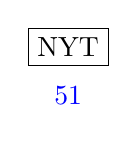
\begin{tikzpicture}
        \tikzstyle{every node}=[circle,draw]
        \node (Root)[rectangle, label={[blue]below:51}] {NYT};
      \end{tikzpicture}
    \item \textbf{a} encoded:
      \begin{multicols}{2}
        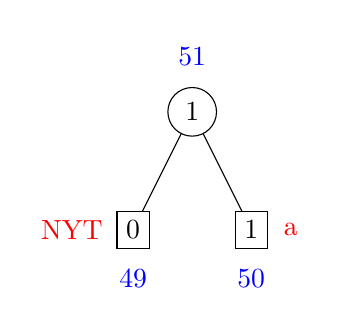
\begin{tikzpicture}
          \tikzstyle{every node}=[circle, draw]
          \node (Root)[label={[blue]above:51}] {1}
          child{
            node[rectangle, label={[red]left:NYT}, label={[blue]below:49}] {0}
          }
          child{
            node[rectangle, label={[red]right:a}, label={[blue]below:50}] {1}
          };
        \end{tikzpicture}
        
        \null \vfill
        \begin{tabular}{ cc } 
          00000 &  \\
          % \hline
          a &  \\
          \end{tabular}

          \null \vfill
      \end{multicols}
    \item \textbf{a a} encoded:
      \begin{multicols}{2}
        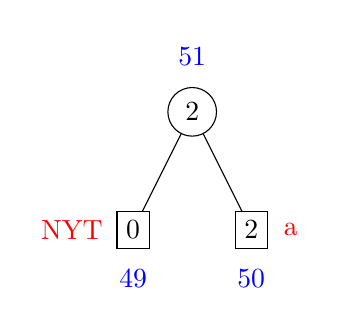
\begin{tikzpicture}
          \tikzstyle{every node}=[circle, draw]
          \node (Root)[label={[blue]above:51}] {2}
          child{
            node[rectangle, label={[red]left:NYT}, label={[blue]below:49}] {0}
          }
          child{
            node[rectangle, label={[red]right:a}, label={[blue]below:50}] {2}
          };
        \end{tikzpicture} \\
        \null \vfill
        \begin{tabular}{ cc } 
          00000 & 1 \\
          % \hline
          a & a \\
          \end{tabular} \\
          \null \vfill
      \end{multicols}
    \newpage
    \item \textbf{a a b} encoded: 
      \begin{multicols}{2}
        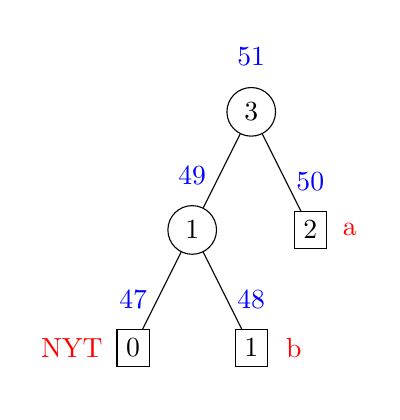
\begin{tikzpicture}
          \tikzstyle{every node}=[circle, draw]
          \node (Root)[label={[blue]above:51}] {3}
          child{
            node[label={[blue]above:49}] {1}
            child{
              node[rectangle, label={[red]left:NYT}, label={[blue]above:47}] {0}
            }
            child {
              node[rectangle, label={[red]right:b}, label={[blue]above:48}] {1}
            }
          }
          child{
            node[rectangle, label={[red]right:a}, label={[blue]above:50}] {2}
          };
        \end{tikzpicture} \\
        \null \vfill
        \begin{tabular}{ cccc } 
          00000 & 1 & 0 & 00001\\
          % \hline
          a & a & NYT & b\\
          \end{tabular} \\
          \null \vfill
      \end{multicols}
    \item \textbf{a a b b} encoded: 
      \begin{multicols}{2}
        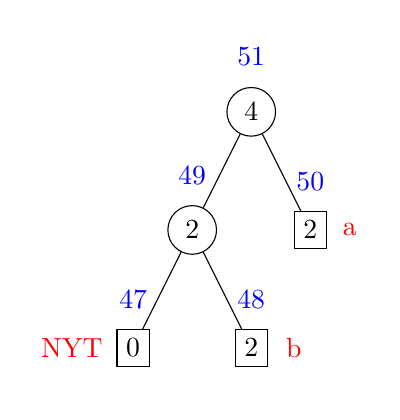
\begin{tikzpicture}
          \tikzstyle{every node}=[circle, draw]
          \node (Root)[label={[blue]above:51}] {4}
          child{
            node[label={[blue]above:49}] {2}
            child{
              node[rectangle, label={[red]left:NYT}, label={[blue]above:47}] {0}
            }
            child {
              node[rectangle, label={[red]right:b}, label={[blue]above:48}] {2}
            }
          }
          child{
            node[rectangle, label={[red]right:a}, label={[blue]above:50}] {2}
          };
        \end{tikzpicture} \\
        \null \vfill
        \begin{tabular}{ ccccc } 
          00000 & 1 & 0 & 00001 & 01\\
          % \hline
          a & a & NYT & b & b\\
          \end{tabular} \\
          \null \vfill
      \end{multicols}
    \item \textbf{a a b b a} encoded:
      \begin{multicols}{2}
        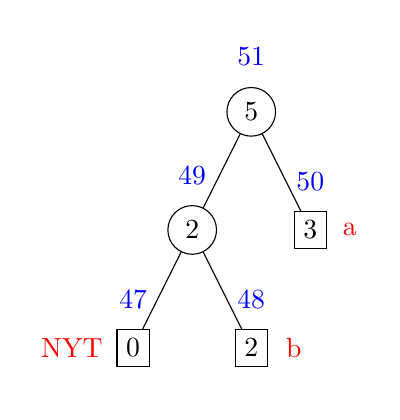
\begin{tikzpicture}
          \tikzstyle{every node}=[circle, draw]
          \node (Root)[label={[blue]above:51}] {5}
          child{
            node[label={[blue]above:49}] {2}
            child{
              node[rectangle, label={[red]left:NYT}, label={[blue]above:47}] {0}
            }
            child {
              node[rectangle, label={[red]right:b}, label={[blue]above:48}] {2}
            }
          }
          child{
            node[rectangle, label={[red]right:a}, label={[blue]above:50}] {3}
          };
        \end{tikzpicture} \\
        \null \vfill
        \begin{tabular}{ cccccc } 
          00000 & 1 & 0 & 00001 & 01 & 1\\
          % \hline
          a & a & NYT & b & b & a\\
        \end{tabular} \\
        \null \vfill
      \end{multicols}
  \end{enumerate}
% \end{multicols}
\newpage
\section*{Problem 6 Golomb Encoding and Decoding.}
\begin{enumerate}[label=(\alph*)]
  \item Find the Golomb code of n=21 when m=4.
  \subsection*{Ans}
    \begin{align*}
      &2^{\ceil*{\log_2^{m}}}-m=2^{2}-4 = 0 \\
      &encoded~21 = 21/4 = 5 \dots 1 = 111110~01 
    \end{align*}
  \item Find the Golomb code of n=14 when m=4.
  \subsection*{Ans}
  \begin{align*}
    &2^{\ceil*{\log_2^{m}}}-m=2^{2}-4 = 0 \\
    &encoded~14 = 14/4 = 3 \dots 2 = 1110~10 
  \end{align*}
  \item Find the Golomb code of n=21 when m=5.
  \subsection*{Ans}
    \begin{align*}
      &2^{\ceil*{\log_2^{m}}}-m=2^{3}-5 = 3 \\
      &encoded~21 = 21/5 = 2 \dots 1 = 110~01 
    \end{align*}
  \item Find the Golomb code of n=14 when m=5.
  \subsection*{Ans}
    \begin{align*}
      &2^{\ceil*{\log_2^{m}}}-m=2^{3}-5 = 3 \\
      &encoded~14 = 14/5 = 2 \dots 4 = 110~111 
    \end{align*}
  \item A two-integer sequence is encoded by Golomb code with m=4 to get the bitstream
  11101111000. What’s the decoded two-integer sequence?
  \subsection*{Ans}
    \begin{align*}
      &2^{\ceil*{\log_2^{m}}}-m=2^{2}-4 = 0 \\
      &\begin{tabular}{ cccc } 
        \underline{1110} & \underline{11} & \underline{110} & \underline{00} \\
        3                & 3              & 2               & 0 \\
      \multicolumn{2}{c}{15} & \multicolumn{2}{c}{8}
      \end{tabular} \\
    \end{align*}
  \newpage
  \item A two-integer sequence is encoded by Golomb code with m=5 to get the bitstream
  11101111000 (the same bitstream as that in (e)). What’s the decoded two-integer sequence?\\
  \textbf{Hint}: The unary code for a positive integer q is simply q 1s followed by a 0.
  \subsection*{Ans}
  \begin{align*}
    &2^{\ceil*{\log_2^{m}}}-m=2^{3}-4 = 4 \\
    &\begin{tabular}{ cccc } 
     \underline{1110} & \underline{11} & \underline{110} & \underline{00} \\
     3                & 3              & 2               & 0 \\
    \multicolumn{2}{c}{18} & \multicolumn{2}{c}{10}
    \end{tabular} \\
  \end{align*}
\end{enumerate}
\end{document}